\documentclass[11pt,a4paper]{article}
\usepackage[margin=1in]{geometry}

% The preceding line is only needed to identify funding in the first footnote. If that is unneeded, please comment it out.
\usepackage{cite}
\usepackage{amsmath,amssymb,amsfonts}
\usepackage{graphicx}
\usepackage{textcomp}
\usepackage{xcolor}
\usepackage[english]{babel}
\usepackage[utf8]{inputenc}
\usepackage[hidelinks]{hyperref}
\usepackage[table]{xcolor}
% \usepackage{url}
% \usepackage{svg}
\usepackage{caption}
\usepackage{float}
% \usepackage{hyperref}
% \usepackage{url}
\usepackage[acronym]{glossaries}
\usepackage[font=footnotesize,labelfont=bf,labelsep=colon]{caption}

\usepackage{algorithm}
% \usepackage{algorithmic}
\usepackage{algpseudocode}

\usepackage{hyperref}
\usepackage{xurl}

\makeatletter
\patchcmd{\@verbatim}
  {\verbatim@font}
  {\verbatim@font\small}
  {}{}
\makeatother

\makeglossaries

\begin{document}

\title{Evolutionary Computation\\CA2 Report}
\author{
Joseph Haines\\
\small{Student ID: 2327945}
}

\maketitle

% \tableofcontents

\section*{Exercise 4}
\label{sec:exercise-4}

% Describe your algorithm from Exercise 3 in the form of pseudo-code (see Lab 1 for an example).
% The pseudo-code should be su!ciently detailed to allow an exact re-implementation.

% \texttt{def evolutionary\_algorithm(n: int, m: int, clauses: List[List[int]], time\_budget: int, **kwargs):}

$\mu,\lambda$ Binary Genetic Algorithm with Crossover for MAX-SAT Optimisation \\
\textit{Python Implementation: \texttt{./common/maxsat.py}}

\noindent
\begin{verbatim}

// Input variables
let n           = number of variables
let m           = number of clauses
let clauses     = list of clauses
let time_budget = maximum amount of time (in seconds) allowed for the algorithm to run

// Algorithm parameters
mu_count        <- 5
lambda_mu_ratio <- 6
crossover_prob  <- 0.85
mutation_prob   <- 1 / n
lambda_count    <- mu_count * lambda_mu_ratio

start <- time_s()             // store start time
end   <- start + time_budget  // pre-compute end time

// Initialise Random Population
population <- empty set
for i <- [1..mu_count]
  population[i] <- uniformly random list of integers from {0,1} of size n
end for

// Main Loop
generation <- 0
xbest      <- empty
nsat       <- -1
while time_s() <= end

  generation <- generation + 1

  // select lambda_count offspring
  offspring <- empty set
  for i <- [1..lambda_count]
    offspring[i] <- random individual from population
  end for

  // apply crossover
  for i <- [1,3,5,...,lambda_count-1]  // step by 2
    if rand() < crossover_prob
      o_1, o_2         <- offspring[i], offspring[i+1]
      crossover_point  <- rand([1..n-1]) // random int between 1 and n-1
      offspring[i]     <- concat(o_1[1:crossover_point], o_2[crossover_point+1:n])
      offspring[i+1]   <- concat(o_2[1:crossover_point], o_1[crossover_point+1:n])
    end if
  end for

  // apply mutation
  for i <- [1..lambda_count]
    for j <- [1..n]
      if rand() < mutation_prob
        offspring[i][j] <- offspring[i][j] ^ 1
      end if
    end for
  end for

  // calculate offspring costs
  costs <- empty set
  for i <- [1..lambda_count]
    individual        <- offspring[i]
    satisfied_clauses <- 0
    for each clause in clauses
      clause_satisfied <- false
      for each literal in clause
        value    <- individual[abs(literal)]
        if literal < 0
          value <- value ^ 1
        end if
        if value == 1
          clause_satisfied <- true
        end if
      end for
      if clause_satisfied
        satisfied_clauses <- satisfied_clauses + 1
      end if
    end for
    costs[i] <- satisfied_clauses
  end for

  // truncation selection
  idxs       <- sort_desc(costs)[1:mu_count] // select mu_count best solutions
  population <- offspring[idxs]

  // update record of best individual
  best_offspring <- offspring[idxs[1]]
  best_nsat      <- costs[idxs[1]]
  if best_nsat > nsat
    xbest <- best_offspring
    nsat  <- best_nsat
  end if

  // if we've covered every row, we can exit early.
  if best_nsat == m
    break while
  end if

end while

t <- generation * mu_count
return t,nsat,xbest

\end{verbatim}



% \begin{algorithm}
% \caption{Heuristic improvement operator for the SPP}
% \begin{algorithmic}[1]

% \State \textbf{Let}:
% % $\begin{cases}
% % n = \text{number of variables} \\
% % m = \text{number of clauses in benchmark} \\
% % clauses = \text{the set of clauses} i,\ i \in I \text{ in } S.
% % \end{cases}$

% % \State initialise $w_i := |\alpha_i \cap S|$, $\forall i \in I$;
% % \State set $T := S$; \texttt{/* T is a dummy set */}
% % \Repeat\ \texttt{/* DROP procedure */}
% %     \State randomly select a column $j,\ j \in T$ and set $T \leftarrow T - j$;
% %     \If{$w_i \geq 2$, for any $i \in \beta_j$}
% %         \State set $S \leftarrow S - j$; set $w_i \leftarrow w_i - 1$, $\forall i \in \beta_j$;
% %     \EndIf
% % \Until{$T = \emptyset$};
% % \State initialise $U := \{i \mid w_i = 0,\ \forall i \in I\}$;
% % \State set $V := U$; \texttt{/* V is a dummy set */}
% % \Repeat\ \texttt{/* ADD procedure */}
% %     \State randomly select a row $i \in V$ and set $V \leftarrow V - i$;
% % \Until{$V = \emptyset$};   % <-- ADD THIS LINE

% \end{algorithmic}
% \end{algorithm}

\section*{Exercise 5}
\label{sec:exercise-5}

% Your algorithm is likely to have several parameters, such as the population size, that must be set be-
% fore running the algorithm. Choose three parameters which you think are essential for the behaviour
% of your algorithm. Run a set of experiments to determine the impact of these parameters on the
% quality (number of satisfied clauses) of the solutions obtained. For each parameter setting, run the
% algorithm on some selected problem instances from the MAXSAT competition (MSE17 complete
% unweighted benchmarks) which you can download from the following URL:
% http: // mse17. cs. helsinki. fi/ benchmarks. html
% Note that some of the instances in the MAXSAT competition are very large. Unless you have a
% significant computational resources available, you might find it useful to start with the smallest
% instances. You will also need to set a reasonable time out value that allows you to run a su!cient
% number of experiments.
% For each parameter setting and problem instance, make 100 repetitions. Plot the results as boxplots,
% and discuss your findings. Clearly indicate which of the instances you tested your code on.

\noindent Three parameters were chosen to run experiments against:
\begin{itemize} \parskip0pt \parsep0pt
  \item \textbf{\texttt{lambda\_mu\_ratio}}: The ratio of $\lambda:\mu$ (where $\mu = 5$)
  \item \textbf{\texttt{crossover\_prob}}: The probability of applying a single-point crossover between 2 offspring
  \item \textbf{\texttt{mutation\_prob}}: The probability of flipping a single bit in the binary representation of an individual
\end{itemize}

\noindent For all three parameters, the same three benchmark instances were used:
% MSE17 complete unweighted benchmarks http://mse17.cs.helsinki.fi/benchmarks.html
\begin{itemize} \parskip0pt \parsep0pt
  \item \texttt{bcp-fir/normalized-fir06\_area\_delay.wcnf}
  \item \texttt{reversi/rev66-4.wcnf}
  \item \texttt{pbo-mqc-nencdr/10tree305p.wcnf}
\end{itemize}


\subsection*{Experiments: \texttt{lambda\_mu\_ratio}}

For the experiments modulating the \texttt{lambda\_mu\_ratio} parameter, the following values were chosen:
\begin{flushleft}
  \begin{tabular}{|c|c|c|c|c|c|c|c|c|c|}
  \hline
  % 2,3,4,5,6,7,8,9,10
  \textbf{\texttt{lambda\_mu\_ratio}} & 2 & 3 & 4 & 5 & 6 & 7 & 8 & 9 & 10 \\
  \hline
  \end{tabular}
\end{flushleft}

For each parameter setting, 100 independent trials were performed with a 5 second time limit per trial. The figure reports the resulting boxplots, split by benchmark instance.

\begin{figure}[!h]
  \centering
  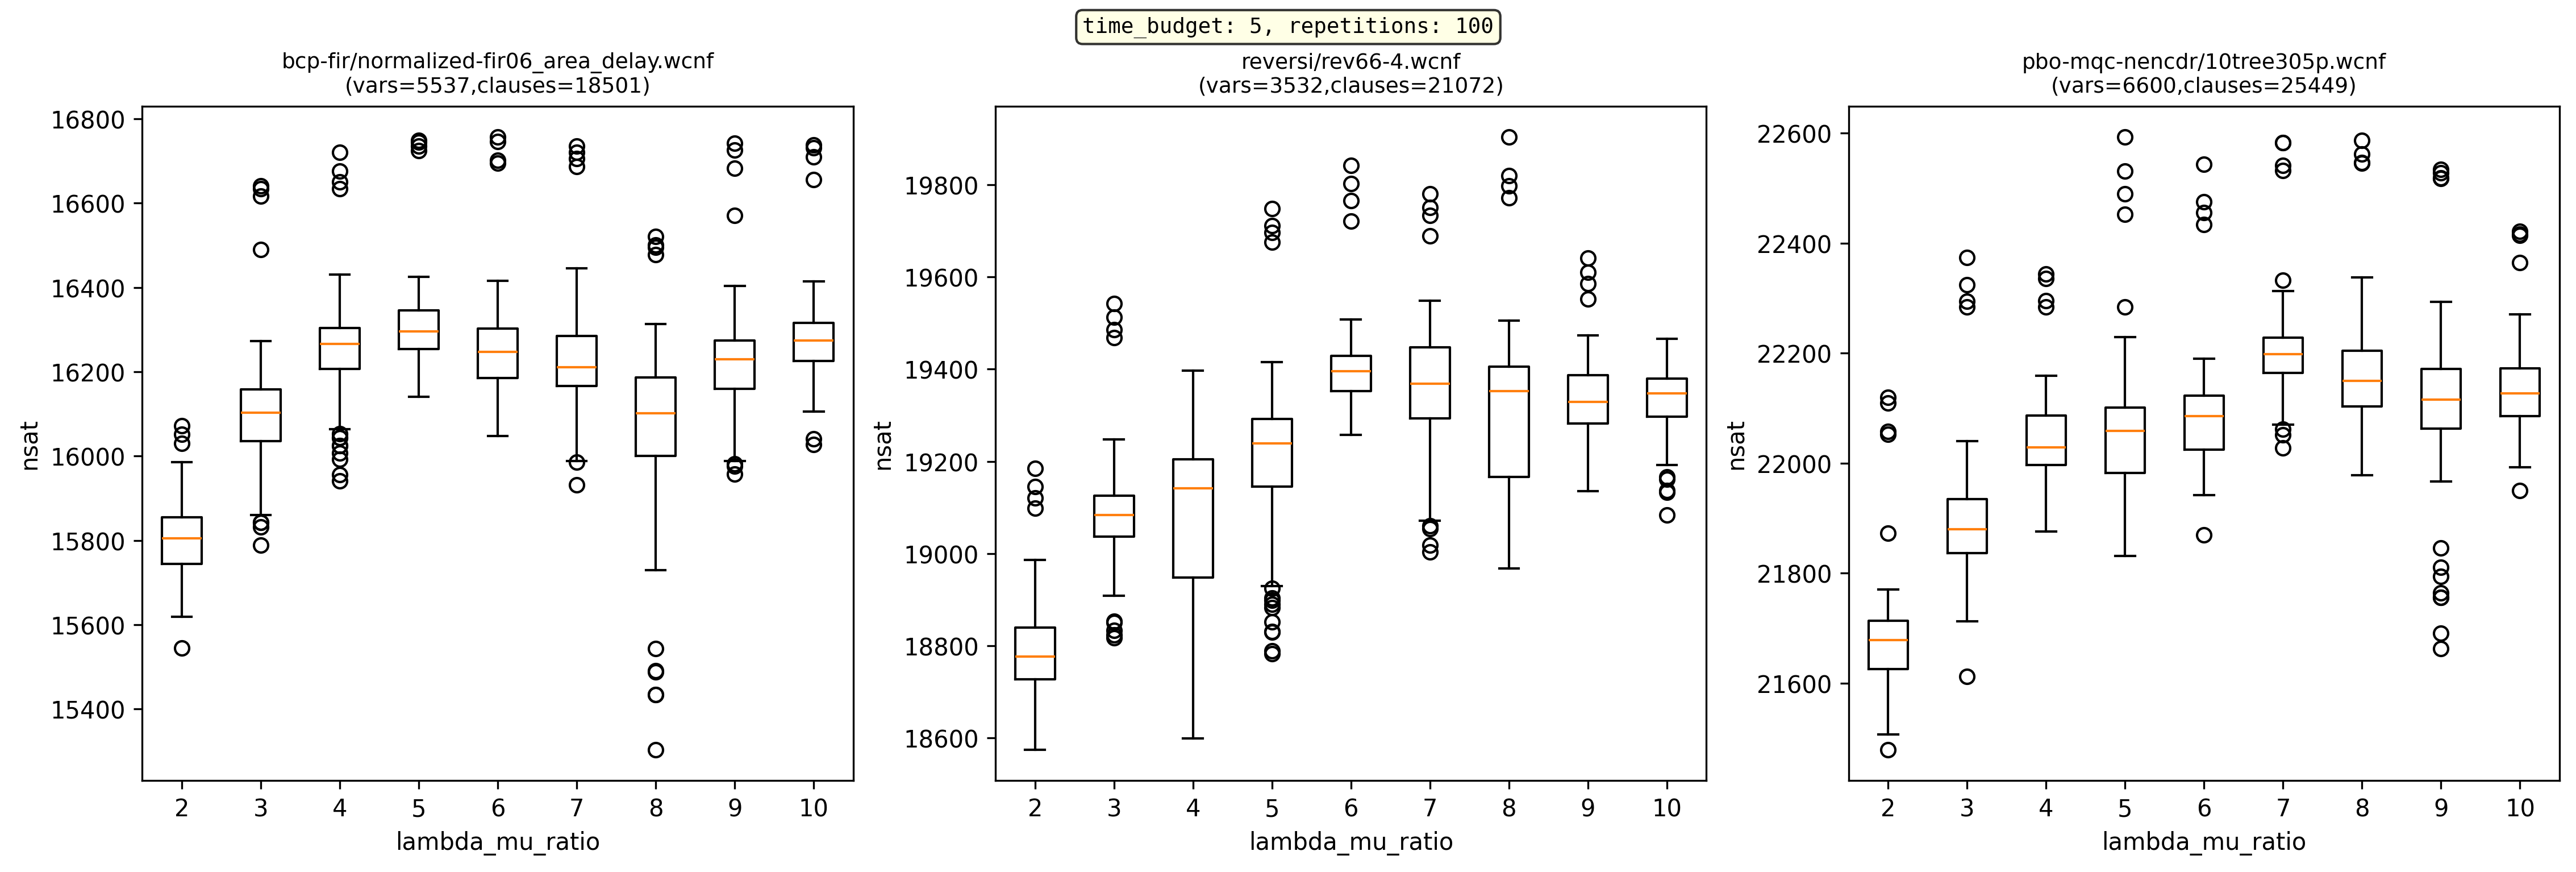
\includegraphics[width=\textwidth]{exercise5/output/lambda_mu_ratio/lambda_mu_ratio_5s_100x_normalized-fir06_area_delay_rev66-4_10tree305p.png}
  \caption{\texttt{lambda\_mu\_ratio} trial results}
\end{figure}

\noindent \textbf{Discussion:} \\
The results from the above trials show that increasing the \texttt{lambda\_mu\_ratio} improves solution quality up to a point, beyond which further increases yield diminishing returns. Across all three benchmark instances, performance is lowest at ratio 2 and improves notably when ratio is increased to 3, and again when increased to 4. From ratio 5 onwards, the median solution quality plateaus, with minimal improvement at higher ratios (7--10). This suggests that the additional selection pressure from larger offspring pools provides substantial benefit initially by allowing better parents to be selected, but eventually the marginal improvement becomes negligible. 

However, the plateauing effect may also be influenced by the fixed time budget. Higher \texttt{lambda\_mu\_ratio} values require generating and evaluating more offspring per generation, which increases computational cost per iteration. Under this time limit, higher ratios result in fewer total generations completed, offsetting the potential benefits of stronger selection pressure. This creates a trade-off where larger offspring pools appear to improve solution quality per generation, but fewer generations can be executed within the time bound. The consistent pattern across all instances indicates that a ratio of 5--6 represents a reasonable balance between computational cost and quality gain, accounting for both the selection benefit and the generational cost. Existing academic research typically suggests a value of $\sim$7 for the $\lambda:\mu$ ratio, which these experiments support within a margin of problem and implementation-specific variation.

\subsection*{Experiments: \texttt{crossover\_prob}}

For the experiments modulating the \texttt{crossover\_prob} parameter, the following values were chosen:
\begin{flushleft}
  \begin{tabular}{|c|c|c|c|c|c|c|c|c|c|}
  \hline
  % 0,0.1,0.5,0.75,0.8,0.85,0.9,0.95,1
  \textbf{\texttt{crossover\_prob}} & 0 & 0.1 & 0.5 & 0.75 & 0.8 & 0.85 & 0.9 & 0.95 & 1 \\
  \hline
  \end{tabular}
\end{flushleft}

For each parameter setting, 100 independent trials were performed with a 5 second time limit per trial. The figure reports the resulting boxplots, split by benchmark instance.

\begin{figure}[!h]
  \centering
  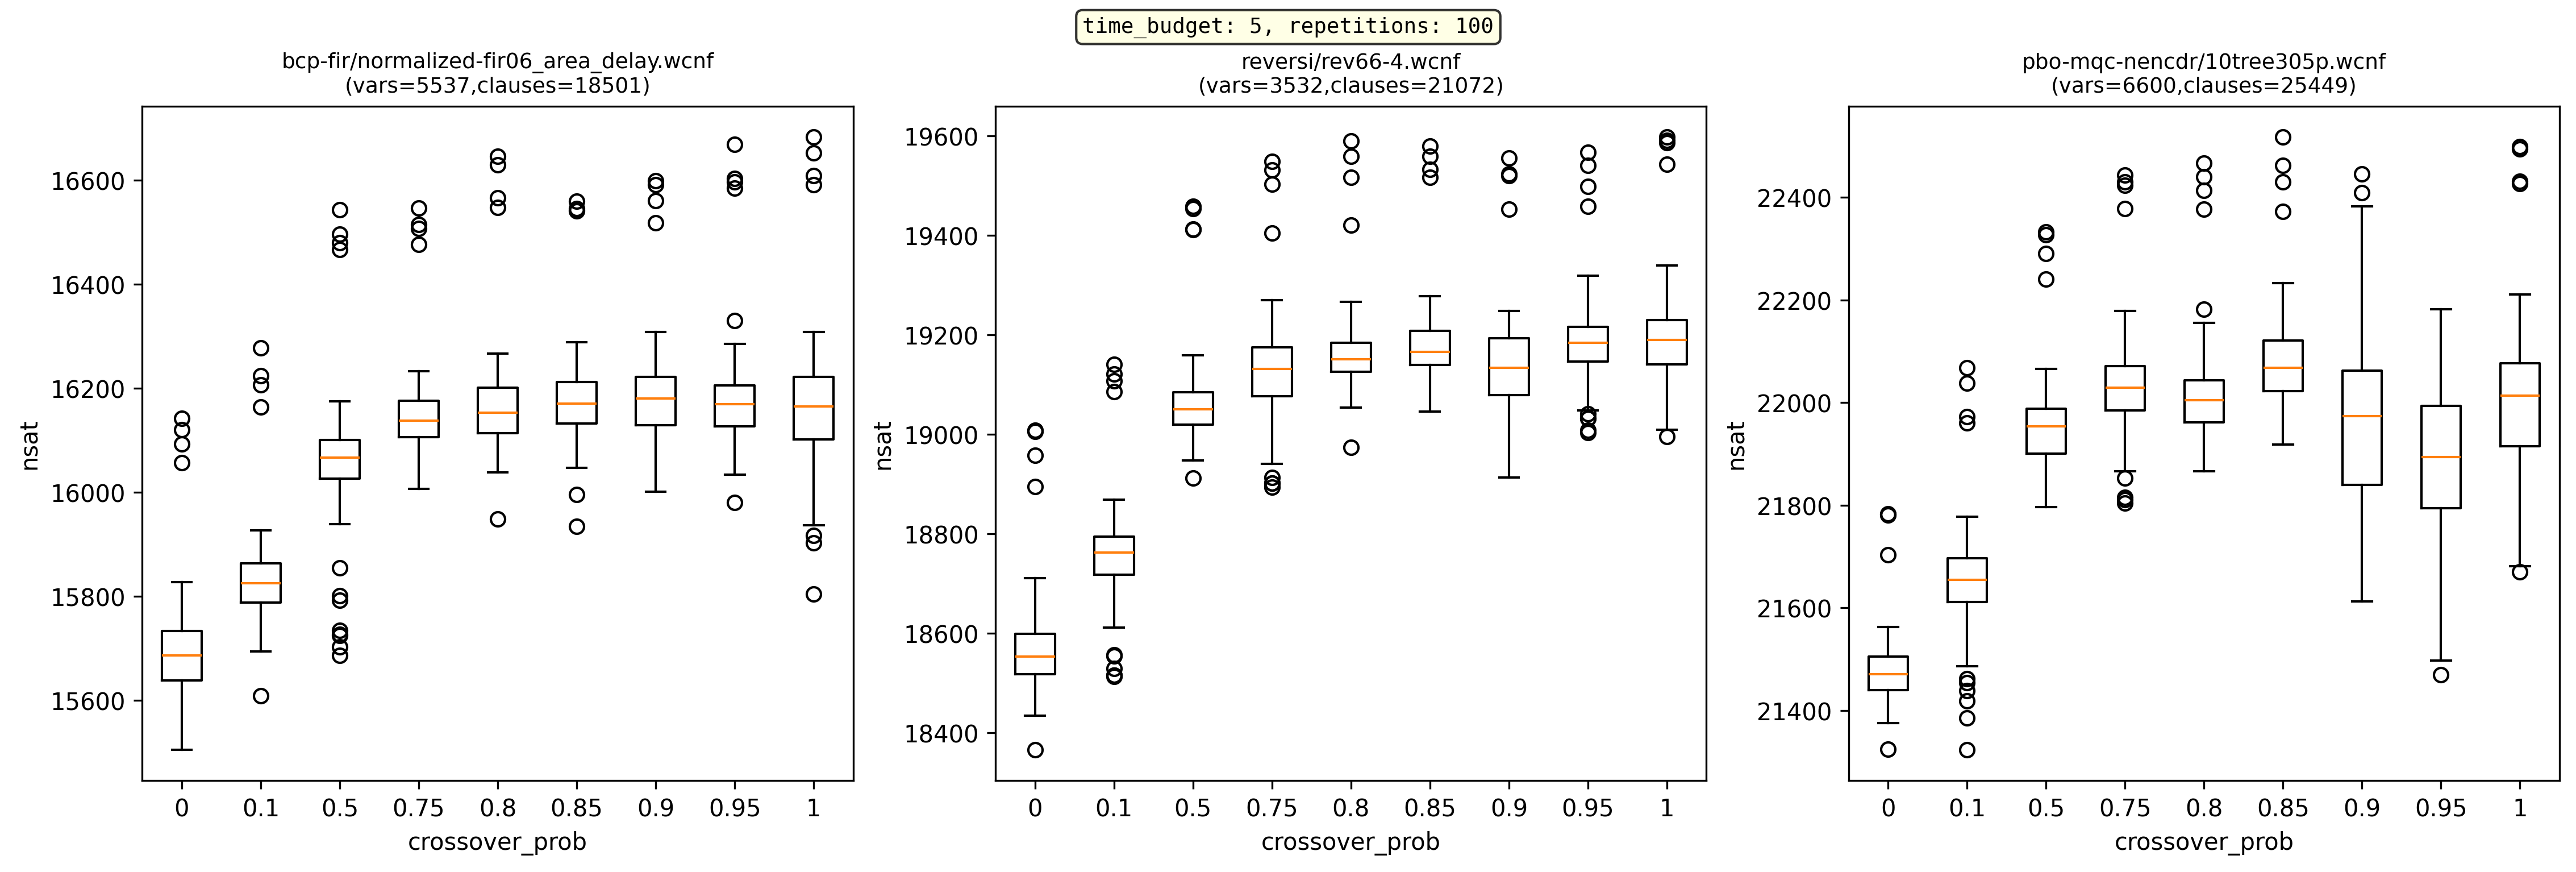
\includegraphics[width=\textwidth]{exercise5/output/crossover_prob/crossover_prob_5s_100x_normalized-fir06_area_delay_rev66-4_10tree305p.png}
  \caption{\texttt{crossover\_prob} trial results}
\end{figure}

\noindent \textbf{Discussion:} \\
The results from the above trials show that crossover probability has a clear impact on solution quality, with performance varying substantially across the tested range. At \texttt{crossover\_prob} of 0 (no crossover), all three instances exhibit notably poor solutions, indicating that crossover is beneficial for this problem domain. Performance improves steadily as crossover probability increases from 0, reaching a peak in the range of 0.75--0.85 where median solution quality is best. Beyond 0.75--0.85, increasing the crossover probability further shows either stagnation or slight degradation on some instances.

The base algorithm choice of \texttt{crossover\_prob} = 0.85 aligns well with these experimental results and represents an effective configuration across diverse problem instances.

\subsection*{Experiments: \texttt{mutation\_prob}}

For the experiments modulating the \texttt{mutation\_prob} parameter, the following values were chosen:
\begin{flushleft}
  \begin{tabular}{|c|c|c|c|c|c|c|}
  \hline
  % '1/n','5/n','10/n','15/n','20/n','25/n'
  \textbf{\texttt{mutation\_prob}} & 1/n & 5/n & 10/n & 15/n & 20/n & 25/n \\
  \hline
  \end{tabular}
\end{flushleft}

For each parameter setting, 100 independent trials were performed with a 5 second time limit per trial. The figure reports the resulting boxplots, split by benchmark instance.

\begin{figure}[!h]
  \centering
  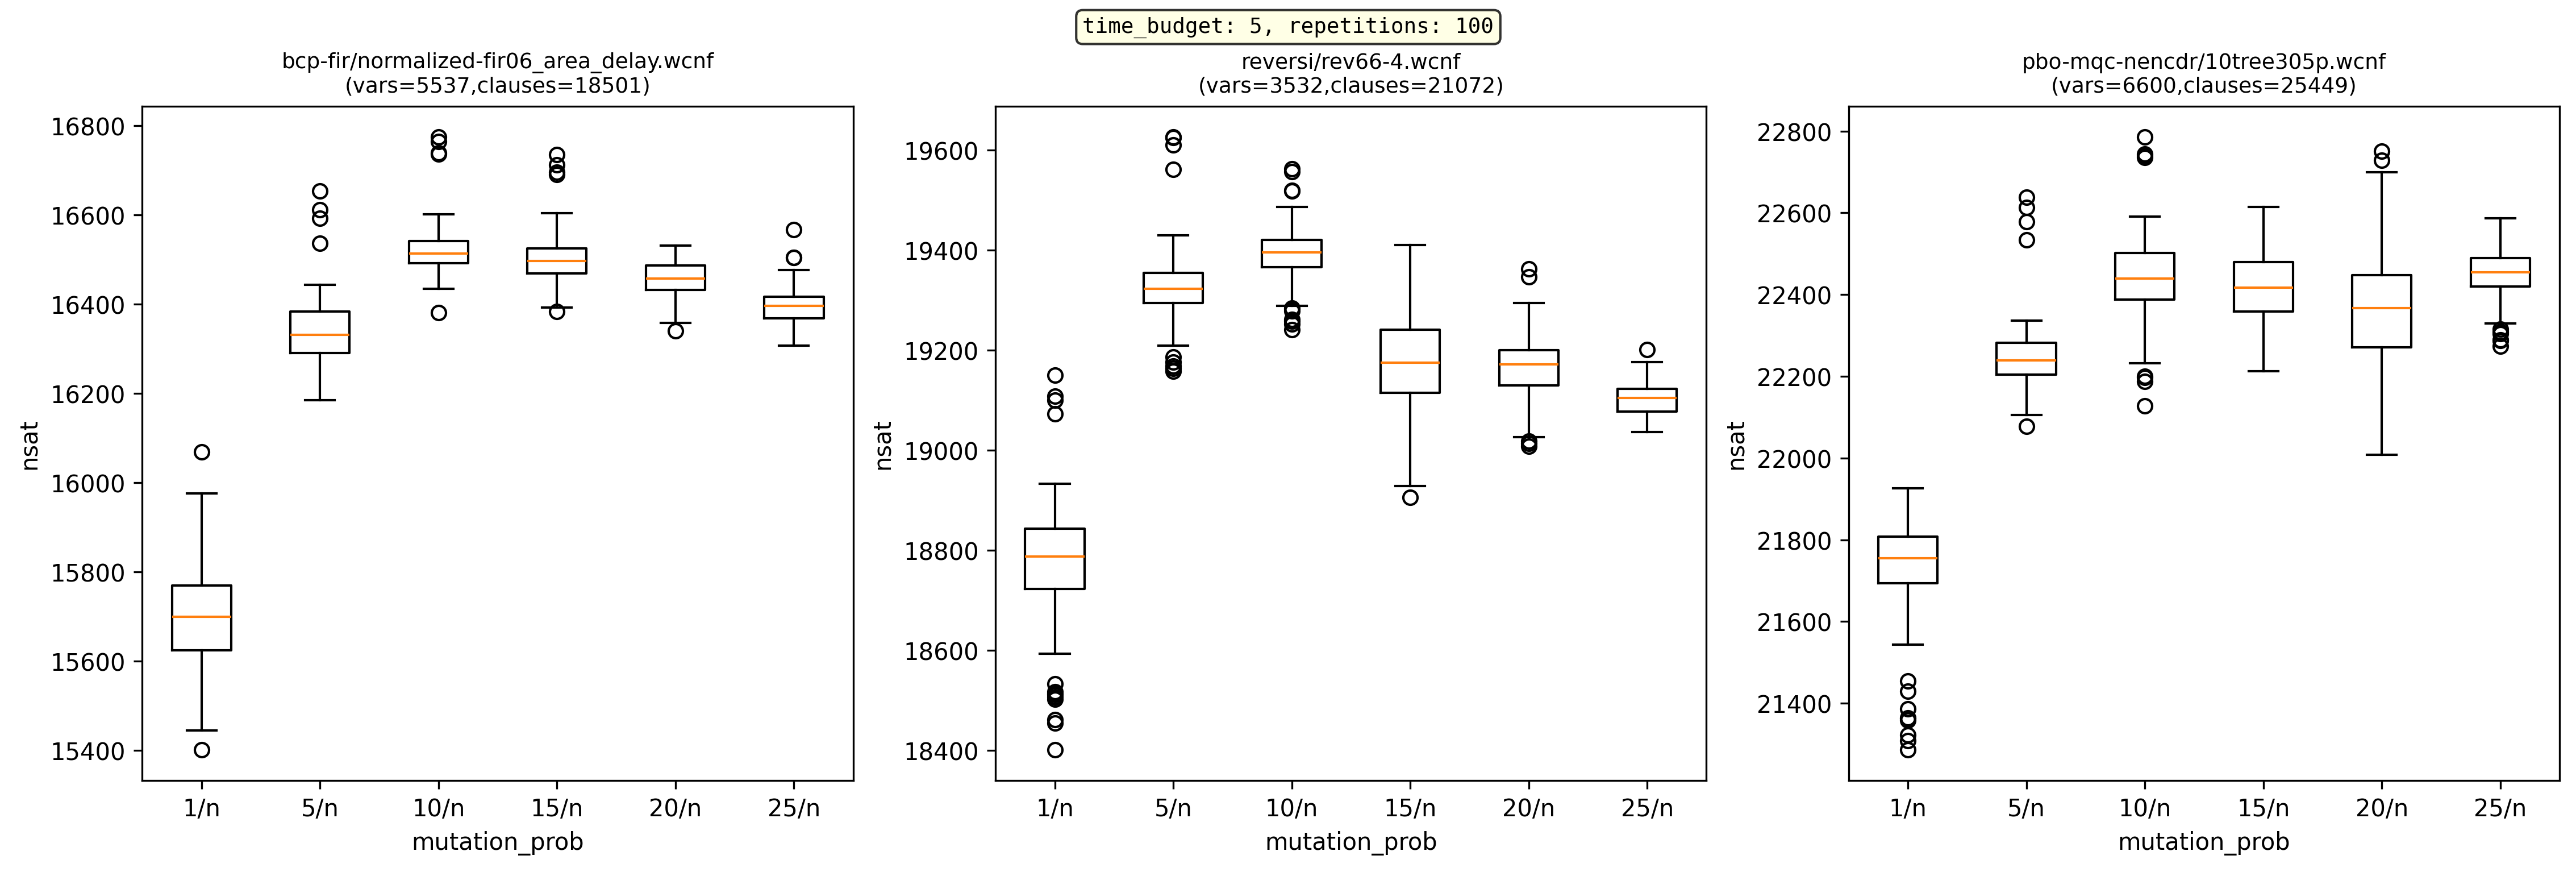
\includegraphics[width=\textwidth]{exercise5/output/mutation_prob/mutation_prob_5s_100x_normalized-fir06_area_delay_rev66-4_10tree305p.png}
  \caption{\texttt{mutation\_prob} trial results}
\end{figure}

\noindent \textbf{Discussion:} \\
The results from the above trials show an unexpected pattern: high mutation probabilities (e.g. 10/n, 15/n, and 20/n) yield better solution quality compared to lower mutation rates (e.g. 1/n, 5/n). This result contradicts conventional wisdom in evolutionary computation, where mutation rate is typically suggested to be set to 1/n. I believe that these results are due to the short 5 second time limit. Within a short time window, higher mutation rates may provide exploration benefits that outweigh their disruptive effects, helping the algorithm escape local optima and sample the search space more thoroughly before time expires. Conversely, lower mutation rates on short time budgets may become too exploitative prematurely, converging to mediocre solutions without sufficient time to refine them.

To confirm this hypothesis, additional experiments were conducted with a longer 20 second time budget on the \texttt{bcp-fir/normalized-fir06\_area\_delay.wcnf} instance (Figure~\ref{fig:mutation_prob_convergence}). The results strongly support the time budget theory: with adequate time, lower mutation rates (1/n and 5/n) significantly outperform higher rates. In contrast, higher mutation rates (15/n, 20/n, 25/n) plateau at lower quality, suggesting they converge to suboptimal solutions faster.

\begin{figure}[!h]
  \centering
  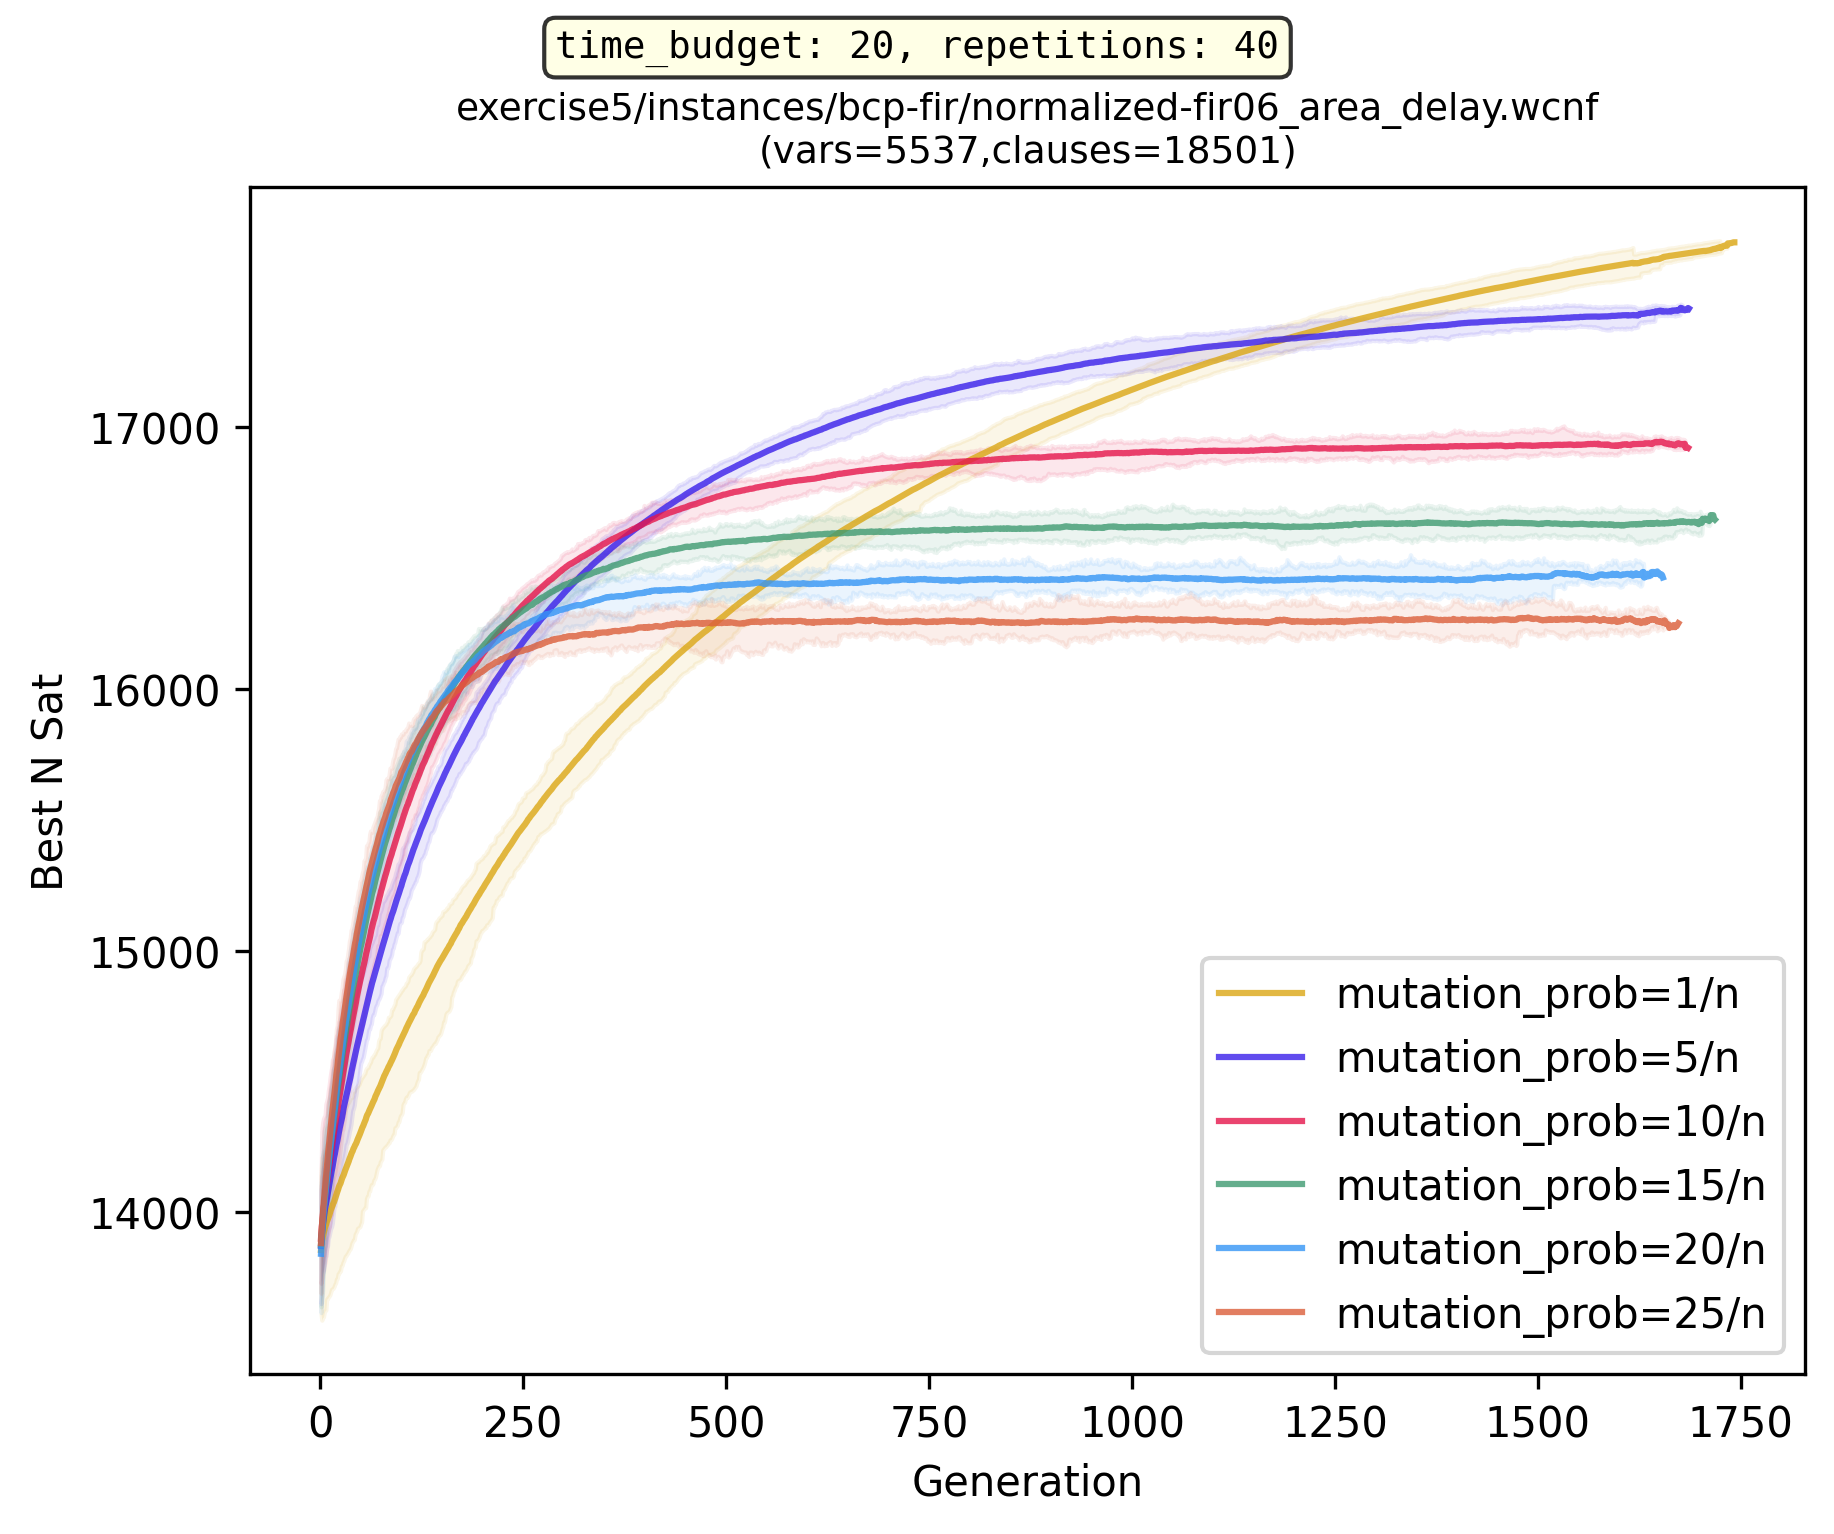
\includegraphics[width=0.5\textwidth]{multi_param_graph/output/mutation_prob/mutation_prob_20s_40x_normalized-fir06_area_delay.png}
  \caption{\texttt{mutation\_prob} convergence over time (20s budget, single instance)}
  \label{fig:mutation_prob_convergence}
\end{figure}

The explanation is clear: with only 5 seconds, the algorithm explores broadly with high mutation but lacks time to refine solutions, making the initial diversity beneficial. With 20 seconds, the extended time allows lower mutation rates to perform refining exploitation, yielding superior final solutions. These findings demonstrate that mutation rate efficacy is highly time-budget dependent. For the 5-second constraint used in the main experiments, a high mutation rate (10/n--15/n) is effective; however, for longer runs with adequate convergence time, the base algorithm's conservative choice of 1/n is indeed optimal.

% \noindent \textbf{Future Direction: Adaptive Mutation Rate} \\
Given the clear time-budget dependency observed, an adaptive mutation strategy that decreases the rate over time could potentially combine the benefits of both regimes. Such an approach would provide high initial population diversity to escape local optima and sample broadly, while transitioning toward lower mutation rates as the time budget approaches exhaustion, allowing exploitation and refinement of promising solutions. This strategy shares conceptual similarity with simulated annealing, which gradually reduces temperature (exploration intensity) over time to balance exploration and exploitation. Such an approach could represent a promising direction for improving this algorithm's performance across time budgets and problem instances.

\end{document}
